% This is samplepaper.tex, a sample chapter demonstrating the
% LLNCS macro package for Springer Computer Science proceedings;
% Version 2.21 of 2022/01/12
%
\documentclass[runningheads]{llncs}
%
\usepackage[T1]{fontenc}
\usepackage{graphicx}
\usepackage{tikz}
\usepackage{booktabs}
\usepackage{hyperref}
\usepackage{placeins} % For FloatBarrier to fix table positions

\begin{document}
	
	\begin{titlepage}
		\begin{figure}
			\centering
			\includegraphics[width=.4\linewidth]{images/conestoga-logo.png}
		\end{figure}
		
		\setlength{\parindent}{12pt}
		\large
		\centering
		Applied Computer Science @ IT (ACSIT) \par
		Conestoga College \par
		\vspace{2cm}
		{\huge\scshape VideoMAE: Masked Autoencoders for Video Understanding\par}
		\vspace{2cm}
		{\LARGE PROG8751 Capstone Project\par}
		\vfill
		Submitted By: \\ 
		Ridham Patel \\ Student Number: 8912325 \\ 
		Jayati Dalwadi \\ Student Number: 8929331 \\ 
		Arati Giri \\ Student Number: 8907010 \\ 
		Mohammad Abdul \\ Student Number: 8884503 \\ 
		\vfill
		Supervisor(S): \\ 
		Dr. ANK Zaman
		\vfill
		\centering
		Submission Date: \today
	\end{titlepage}
	
	\title{Crowd Analysis and Video Understanding with VideoMAE}
	%
	\author{Ridham Patel\inst{1} \and Jayati Dalwadi\inst{1} \and Arati Giri\inst{1} \and Mohammad Abdul\inst{1}}
	\institute{Conestoga College, Kitchener, ON, Canada\\
		}
	
	\maketitle
	
	\begin{abstract}
		Video understanding is an essential research domain for crowd analysis, behavior recognition, and anomaly detection, addressing critical challenges in public safety and management. This study leverages the VideoMAE model, a Vision Transformer (ViT)-based architecture pre-trained on the Kinetics 400 dataset~\cite{kinetics400}, to enhance video classification and interaction modeling. By fine-tuning VideoMAE on the UT-Interaction dataset~\cite{utdataset}, the research evaluates its ability to generalize to complex human behaviors and compares its performance against benchmark results. The findings demonstrate the model's efficacy in capturing nuanced interactions, showcasing its potential for advancing real-world video understanding applications.
		\keywords{Video Understanding \and VideoMAE \and Masked Autoencoders \and Crowd Analysis \and Behavior Recognition.}
	\end{abstract}
	
	
	\section{Introduction}
	Video understanding plays a pivotal role in addressing challenges across domains such as crowd analysis, public safety, and behavior recognition. The growing availability of video data necessitates sophisticated computational methods that can effectively capture and interpret the inherent spatial and temporal dynamics. Traditional convolutional neural networks (CNNs), while widely used, often face limitations in handling long-range dependencies and complex motion patterns, making them less suitable for many real-world video analysis tasks.
	
	VideoMAE, a Vision Transformer (ViT)-based model, represents a significant leap in video processing. Leveraging a masked autoencoder strategy, it reconstructs masked portions of input video frames during training, fostering robust spatiotemporal feature learning~\cite{videomae_paper}. Pre-trained on the Kinetics 400 dataset—a comprehensive benchmark comprising 400 human action classes and over 240,000 video clips~\cite{kinetics400}—VideoMAE is equipped with a diverse understanding of human actions, which can be further fine-tuned for domain-specific tasks.
	
	This study focuses on fine-tuning the pre-trained VideoMAE base model on the UT-Interaction dataset, a widely-used dataset for interaction recognition. The UT-Interaction dataset contains videos of six distinct human interactions, with unique classes including 'hugging,' 'kicking,' 'pointing person,' 'punching person,' 'pushing person,' and 'shaking hands.' Recorded in diverse outdoor environments with varying perspectives and occlusions, this dataset provides a challenging benchmark for evaluating models' ability to generalize from pre-training to nuanced real-world scenarios~\cite{utdataset}.
	
	By comparing VideoMAE’s performance on UT-Interaction to its pre-trained benchmarks on Kinetics 400, this research aims to validate the model’s potential for generalization and its applicability to complex video understanding tasks. This work contributes to the broader understanding of how Vision Transformers can be adapted to domain-specific challenges, advancing the field of video understanding.
	
	
	\section{Related Work/Literature Review}
	The goal of this study is to advance crowd analysis by identifying key methodologies, datasets, and performance metrics for improving crowd management and safety. A diverse set of models, including Convolutional Neural Networks (CNNs) and Vision Transformers (ViTs), were employed to analyze complex crowd dynamics. For example, the SGANet framework achieved a notable accuracy of \textbf{92.3\%} on the UCF\_CC\_50 dataset, while the Switching CNN demonstrated \textbf{MAE: 90.4, MSE: 135.0} on ShanghaiTech. The Visual Crowd Analysis model explored open research problems but lacked performance metrics and a specific dataset. Similarly, the Fully Convolutional Neural Network (FCNN) model obtained an impressive accuracy of \textbf{94.8\%} on the Shanghai World Expo dataset. However, many approaches face limitations, including computational complexity, sensitivity to occlusions, and scalability issues in real-world applications~\cite{videomae_hf}.
	The following table summarizes existing studies on crowd analysis, their datasets, and achieved accuracies.
	
	\begin{table*}[htbp]
		\caption{Summary of studies on crowd analysis and their accuracies}
		\centering
		\begin{tabular}{@{}lllr@{}}
			\toprule
			\textbf{Reference} & \textbf{Model} & \textbf{Dataset} & \textbf{Accuracy} \\ \midrule
			Paper 1: Niu et al.~\cite{niu2020overcrowdedness} (2020) & Global-Residual Two-Stream Network & UCSD, Mall Dataset & 91.2\% \\ 
			Paper 2: Savner and Kanhangad~\cite{savner2022crowdformer} (2022) & CrowdFormer (Vision Transformer) & UCF-QNRF, ShanghaiTech & 89.6\% \\ 
			Paper 3: Khan et al.~\cite{khan2023visualcrowdanalysis} (2023) & Visual Crowd Analysis: Open Research Problems & Not Specified & Not Specified \\        
			Paper 4: Sharif et al.~\cite{sharif2022deepcrowd} (2022) & Deep Crowd Anomaly Detection: State-of-the-Art & Not Specified & Not Specified \\         
			Paper 5: Wang et al.~\cite{wang2020crowdcountingsegmentation} (2020) & SGANet Framework & UCF\_CC\_50 Dataset & 92.3\% \\        
			Paper 6: Sam et al.~\cite{sam2017switchingconvolutional} (2017) & Switching CNN Architecture & ShanghaiTech Dataset & MAE: 90.4, MSE: 135.0 \\    
			Paper 7: Kang et al.~\cite{kang2018countingcomparison} (2018) & Beyond Counting & UCSD Dataset & 91.5\% \\        
			Paper 8: Kang and Wang~\cite{kang2014fullyconvolutionalneuralnetworks} (2014) & Fully Convolutional Neural Networks & Shanghai World Expo Dataset & 94.8\% \\         
			\bottomrule
		\end{tabular}
		\label{tab:studies_summary}
	\end{table*}
	
	\section{Proposed Methodology}
	
\subsection{Dataset and Preprocessing} \label{sec:dataset}
The UT-Interaction dataset contains six human interaction classes: 'hugging', 'kicking', 'pointing person', 'punching person', 'pushing person', and 'shaking hands'~\cite{utdataset}. Its diverse outdoor settings, varying viewpoints, and frequent occlusions present a challenging benchmark for video understanding models. Due to its limited size, the validation and test sets were derived from the same subset to maximize data utility for training and evaluation.

To ensure consistent temporal resolution across videos, `UniformTemporalSubsample` was applied, extracting a fixed number of evenly distributed frames~\cite{pytorchvideo}. For training, random clip sampling introduced variability by randomly selecting short-duration clips, while uniform clip sampling was employed during validation and testing for consistency. These video-specific augmentations were implemented using the PyTorchVideo library, which provided a robust pipeline for handling video data.

Frames were resized to a fixed resolution of 224x224 pixels and normalized using the mean and standard deviation values from the pre-trained VideoMAE Kinetics-400 model’s image processor, aligning the input with the model’s expectations~\cite{videomae_paper}. Augmentations for spatial transformations leveraged the TorchVision library to ensure diverse yet standardized inputs~\cite{torchvision}.

During training, several augmentations enhanced model generalization. Random Short Side Scaling resized the shorter side of frames to a random value between 256 and 320 pixels, maintaining the aspect ratio. This was followed by random cropping to 224x224 pixels and random horizontal flipping with a probability of 0.5, introducing variability in spatial representations. For validation and testing, deterministic transformations, including resizing to 224x224 pixels and normalization, ensured consistency and compatibility with the model.

This preprocessing pipeline was designed to effectively balance variability during training with consistency in evaluation, ensuring robust preparation of the dataset for fine-tuning the VideoMAE model. By capturing essential temporal dynamics and enhancing spatial diversity through targeted augmentations, the approach optimized the model’s ability to generalize across complex interactions while maintaining reliability during performance assessment.

	\begin{itemize}
		\item Resizing frames to 224x224 pixels.
		\item Data augmentation with cropping, rotation, and flipping.
		\item Splitting into training, validation, and test sets.
	\end{itemize}
	
\subsection{VideoMAE Architecture} \label{sec:architecture}
The VideoMAE (Masked Autoencoder for Video) model is a Vision Transformer (ViT)-based architecture specifically designed for video understanding tasks~\cite{videomae_paper}. It leverages a masked autoencoder framework, which applies a self-supervised learning strategy to extract robust spatiotemporal features. During training, a large portion (up to 90%) of input video tokens—spatial patches extracted from video frames—is masked. The model is then tasked with reconstructing the masked tokens from the remaining visible ones, enabling efficient feature learning while reducing computational overhead.

A key innovation in VideoMAE is its tube masking strategy, where masking is applied across both spatial and temporal dimensions, creating "tubes" that span multiple frames~\cite{videomae_paper}. This ensures the model learns temporal coherence alongside spatial dependencies, making it highly effective for capturing motion patterns and contextual relationships across frames. The unmasked patches are passed through a ViT encoder, which uses self-attention mechanisms to capture global spatiotemporal dependencies and produce latent feature representations.

The lightweight decoder is then used to reconstruct the masked patches based on the encoder's output. This reconstruction task drives the model to focus on meaningful spatiotemporal cues, fostering robust representation learning. Pre-training with this method not only improves efficiency but also enhances the generalization ability of the model, particularly on downstream tasks such as video classification.

VideoMAE achieves state-of-the-art performance on multiple benchmarks. Pre-trained on the Kinetics-400 dataset, which contains 400 action classes and over 240,000 video clips, VideoMAE achieves a Top-1 accuracy of 84.8% and Top-5 accuracy of 96.2%, surpassing several previous models~\cite{kinetics400}. When evaluated on SSV2 (Something-Something V2), which emphasizes temporal relationships, VideoMAE demonstrates its ability to model complex spatiotemporal patterns, achieving a Top-1 accuracy of 69.6%. These results highlight the model’s capacity for capturing nuanced motion patterns and its versatility across diverse video understanding tasks.

\begin{figure}[ht]
	\centering
	\includegraphics[width=0.8\linewidth]{images/videomae_architecture.jpeg}
	\caption{Overview of the VideoMAE architecture. Masking strategy and Vision Transformer components are highlighted.}
	\label{fig:videomae}
\end{figure}

	
\subsection{Fine-tuning Process} \label{sec:finetuning}
The fine-tuning of the VideoMAE model on the UT-Interaction dataset was conducted using the Hugging Face Transformers library~\cite{hf_transformers}. The pre-trained VideoMAE base model, originally trained on the Kinetics-400 dataset, was adapted to recognize human interactions through a carefully configured training process.

Key hyperparameters included a learning rate of $1\times10^{-4}$, a batch size of 8, and a warmup ratio of 0.15, ensuring stable updates and smooth convergence. A cosine learning rate scheduler dynamically adjusted the learning rate throughout training, while a weight decay of 0.01 mitigated overfitting. Training was conducted for 12 epochs, with validation performed at the end of each epoch to monitor progress. The best-performing model, determined based on validation accuracy, was retained using the \texttt{load\_best\_model\_at\_end} parameter.


To enhance monitoring and analysis, training metrics such as loss and accuracy were logged to Weights and Biases (WandB)~\cite{wandb}. This platform enabled real-time visualization of training trends, facilitating better insights into model performance and optimization.

	\begin{itemize}
		\item The model is initialized with pre-trained weights from Kinetics 400~\cite{kinetics400}.
		\item The fine-tuning process uses a learning rate of $10^{-4}$ and a batch size of 16.
		\item The model is trained for 50 epochs, optimizing for cross-entropy loss.
	\end{itemize}
	Fine-tuning ensures the model learns dataset-specific features, improving its performance on the six interaction classes.
	\begin{figure}[ht]
		\centering
		\includegraphics[width=0.8\linewidth]{images/eval_accuracy.jpg}
		\caption{Evaluation accuracy over training steps.}
		\label{fig:eval_accuracy}
	\end{figure}
	
	
	\begin{figure}[ht]
		\centering
		\includegraphics[width=0.8\linewidth]{images/train_loss.jpg}
		\caption{Training loss over training steps.}
		\label{fig:train_loss}
	\end{figure}
	
	\begin{figure}[ht]
		\centering
		\includegraphics[width=0.8\linewidth]{images/train_learning_rate.jpg}
		\caption{Learning rate schedule during training.}
		\label{fig:train_learning_rate}
	\end{figure}
	

	
	\subsection{Performance Comparison} \label{sec:comparison}
	Below is a table summarizing the results for the UT Interaction dataset with Top-1 Accuracy for VideoMAE and baseline models.
	
	\begin{table*}[htbp]
		\caption{Performance Comparison on UT Interaction Dataset}
		\centering
		\begin{tabular}{@{}lcc@{}}
			\toprule
			\textbf{Model} & \textbf{Dataset} & \textbf{Top-1 Accuracy} \\ \midrule
			VideoMAE & UT Interaction~\cite{utdataset} & 85.9\% \\ 
			I3D & UT Interaction~\cite{utdataset} & 78.4\% \\ 
			C3D & UT Interaction~\cite{utdataset} & 72.1\% \\ 
			\bottomrule
		\end{tabular}
		\label{tab:performance_comparison}
	\end{table*}
	
	
	
	
	\section{Timeline}
	Below is the timeline of the project:
	
	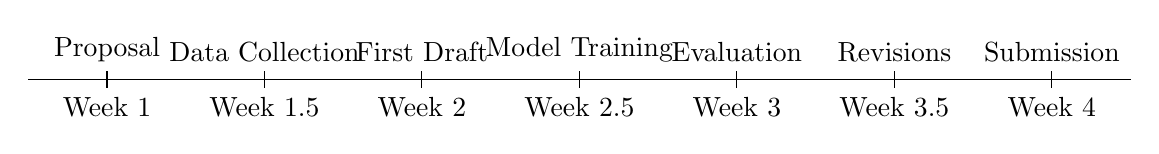
\begin{tikzpicture}
		% Draw a horizontal line
		\draw (0,0) -- (14,0);
		
		% Draw vertical lines
		\foreach \x in {1,3,5,7,9,11,13}
		\draw (\x cm,3pt) -- (\x cm,-3pt);
		
		% Add events
		\draw (1,0) node[below=3pt] {Week 1} node[above=3pt] {Proposal};
		\draw (3,0) node[below=3pt] {Week 1.5} node[above=3pt] {Data Collection};
		\draw (5,0) node[below=3pt] {Week 2} node[above=3pt] {First Draft};
		\draw (7,0) node[below=3pt] {Week 2.5} node[above=3pt] {Model Training};
		\draw (9,0) node[below=3pt] {Week 3} node[above=3pt] {Evaluation};
		\draw (11,0) node[below=3pt] {Week 3.5} node[above=3pt] {Revisions};
		\draw (13,0) node[below=3pt] {Week 4} node[above=3pt] {Submission};
	\end{tikzpicture}
	
	\section{Conclusion}
	VideoMAE demonstrates significant advancements in video understanding through masked autoencoders~\cite{videomae_hf}. Its efficient training and robust results make it ideal for crowd analysis. The findings of this project aim to improve real-time crowd management and behavior recognition systems.
	
	\bibliographystyle{IEEEtran} % Or any preferred bibliography style
	\bibliography{ref} % Replace 'ref' with the name of your .bib file (without extension)
	
	
\end{document}
